This Section describes which steps should be made in order to deploy one or more of the produced models in a real network environment.

\subsection{Sensors}

In order to deploy an IDS in a real network, the first components we need are sensors that are able to record traffic and produce the tuples that will be then fed into the aforementioned model.

Sensor placement is a key factor in an IDS to be able to protect the network from invasion. For this task, the network architecture should be studied in detail, to observe all possible points of entrance.
Depending on how large and complex is our network, we can choose to deploy the whole system in a single device, as suggested by \cite{dpl}, or implement multiple sensors as done in \cite{dpl2}.

In both cases, the most sensitive points where to place the sensors are typically before and after each router or DMZ of the network. Figure~\ref{fig:dpl} describes this situation.

\begin{figure}[h]
    \centering
    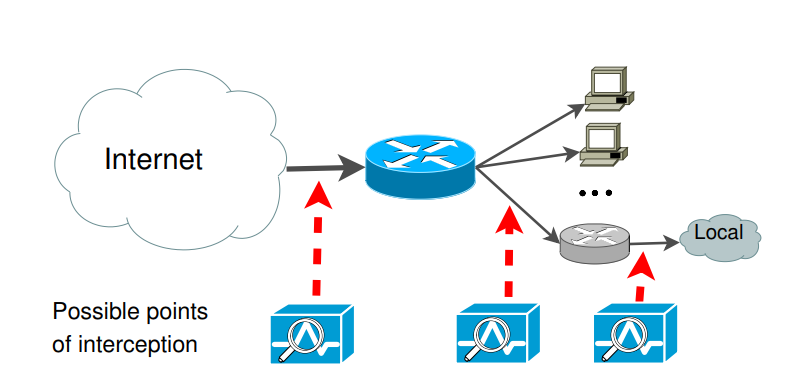
\includegraphics[width=\linewidth]{img/dpl.png}
    \caption{Possible points of interception for a NIDS}
    \label{fig:dpl}
\end{figure}

Generally, IDS sensors have two network interfaces — one for monitoring traffic and one for management. The traffic-monitoring interface is unbound from any protocol, which means that the interface has no IP address and other entities can't communicate with it. This guarantees that no attack surface is exposed on the network by the sensor itself.

\subsection{Model Choice}

After deploying the sensors, we have to choose which model to deploy. The model choice can depend on evaluation metrics like Detection Rate or False Alam Rate, but should also take into account the model complexity. A higher model complexity can in fact imply a higher cost for data acquisition and higher delays for the system's response. This kind of analysis shall be done taking into consideration also the time of response of each model, which is out of the scope of this work.

For reducing the complexity we can employ one of the Feature Selection methods described in Section~\ref{chapter:feature-selection}.

\subsection{Model Deployment}

Once the IDS is deployed in the network, we want it to work with streams of incoming data in a fully automated way. This implies several steps, which are described in Figure~\ref{fig:dplsteps}.

\begin{figure}[h]
    \center
    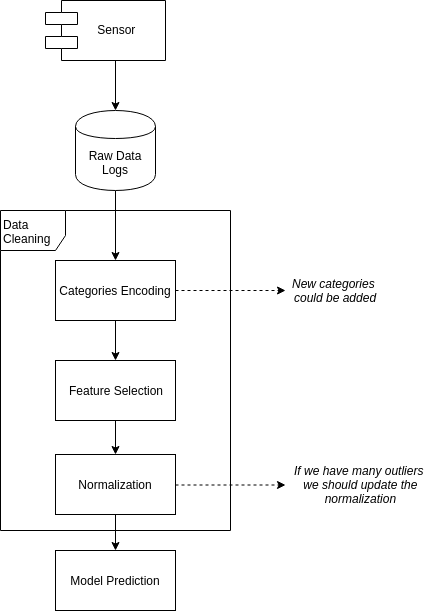
\includegraphics[width=\linewidth]{img/ids-dpl.png}
    \caption{Steps of the IDS once deployed}
    \label{fig:dplsteps}
\end{figure}

There are many possible solutions, to achieve this automation, which range from fully personalized solutions to fully COTS products. One simple possibility, since the models of this work have been trained using TensorFlow, is to use TensorFlow \textit{Extend} \cite{tfx}, a collection of tools used for deploying ANN models in the wild. Figure~\ref{fig:tfx} describes the components of the TFX framework, which range from data cleaning to Keras model validation.

\begin{figure}[h]
    \centering
    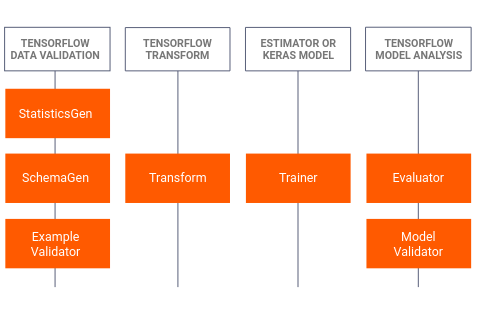
\includegraphics[width=\linewidth]{img/tfx.png}
    \caption{Image taken from \url{https://www.tensorflow.org/tfx/guide}}
    \label{fig:tfx}
\end{figure}

On-Line deployment can be achieved by using \textit{TensorFlow Serving} \cite{tfserve}, which is a framework built to enable fast TensorFlow models' deployment over REST APIs. TF Serving also has the possibility to deploy an ML model in a Docker image and use Kubernetes to manage a cluster of these images running together. This offers a good solution in terms of scalability of the IDS, which is able to easily keep up with a possible growth of the network that it's protecting.

\subsection{Model Adaptation}

Once it is online, the model should be then trained and updated with real data coming from the network. This is a time-consuming task, which requires the network to be in a temporary 'safe' state in which the model can learn which is the normal behaviour of the system. After the training time, the IDS is ready to be used in the network environment.

To extend the training time, a human supervisor can be assigned to checking the entries that are signaled as \textit{anomalous} and relabelling them if necessary. The same model can also be periodically retrained with a larger dataset or with only the latest entries.